% 
%            ,,                                        
%          `7MM            _.o9                                
%            MM                                             
%  ,6"Yb.    MM  ,p6"bo   ,6"Yb.  M"""MMV  ,6"Yb.  `7Mb,od8 
% 8)   MM    MM 6M'  OO  8)   MM  '  AMV  8)   MM    MM' "' 
%  ,pm9MM    MM 8M        ,pm9MM    AMV    ,pm9MM    MM     
% 8M   MM    MM YM.    , 8M   MM   AMV  , 8M   MM    MM     
% `Moo9^Yo..JMML.YMbmd'  `Moo9^Yo.AMMmmmM `Moo9^Yo..JMML.   
% 
% 
% Free and Open-Source template for academic works
% https://github.com/dpmj/alcazar


% Example of an appendix


\chapter{Something vaguely related to the main content, but you put a lot of effort into it.}


\section{Praesent vulputate tellus vel metus rutrum}


Lorem ipsum dolor sit amet, consectetur adipiscing elit. Integer tempus quis elit id sagittis. Cras tincidunt nisi at tellus luctus, et congue dolor posuere. Aliquam suscipit felis sit amet lacus ultrices aliquet. Sed sagittis ultrices nisi, vel elementum elit dignissim non. Fusce faucibus ex at massa ultrices elementum. Nullam ullamcorper lorem sit amet facilisis cursus. Suspendisse non erat non justo porta placerat. Morbi porttitor dictum molestie. Sed vitae iaculis libero. Suspendisse in gravida lacus, tempor ultrices nibh. Nam consequat scelerisque porttitor \cite{europa_rohs, europa_ce}.


\subsection{Faucibus interdum nisi}

Nulla elementum orci in dolor dapibus, ac facilisis sem ultrices. Nullam eleifend id eros sed luctus. Maecenas arcu ipsum, scelerisque id lorem in, placerat posuere tellus \cite{proceedings_piezo}. Etiam gravida velit sed arcu viverra dapibus. Mauris vitae augue dapibus, molestie justo eget, condimentum ipsum. Nulla tristique mi eget semper luctus. Etiam commodo vestibulum vulputate. Etiam quis sapien dolor. Nunc tristique eu lacus quis ullamcorper. Sed volutpat rutrum vehicula. Donec nunc nisl, suscipit in faucibus vitae, tristique eu risus. \glsname{GNU} nulla facilisis augue eget interdum rutrum. Aliquam sem nunc, fermentum sed urna ac, faucibus interdum nisi.


\subsection{Praesent vulputate tellus vel metus rutrum}

Proin a condimentum nibh. Praesent vulputate tellus vel metus rutrum, non luctus mi sollicitudin. Nam ac tellus ut eros sollicitudin luctus at ac mi. Vestibulum mollis nec nisi a laoreet. Proin neque tortor, placerat nec suscipit sit amet, ullamcorper in sem. Fusce faucibus ultrices cursus. Maecenas scelerisque mauris diam, at volutpat nisi porta vitae. 

Sed at ipsum et leo cursus varius eu eu lectus. Class aptent taciti sociosqu ad litora torquent per conubia nostra, per inceptos himenaeos. 

Ut felis ipsum, imperdiet rhoncus orci ac, consectetur luctus nisl. Cras aliquet elementum tellus ullamcorper malesuada. Integer purus est, pharetra eu ullamcorper quis, imperdiet non turpis. \cite{SOFTWARE_ENGINEERING_9}




\begin{figure}
    \centering
    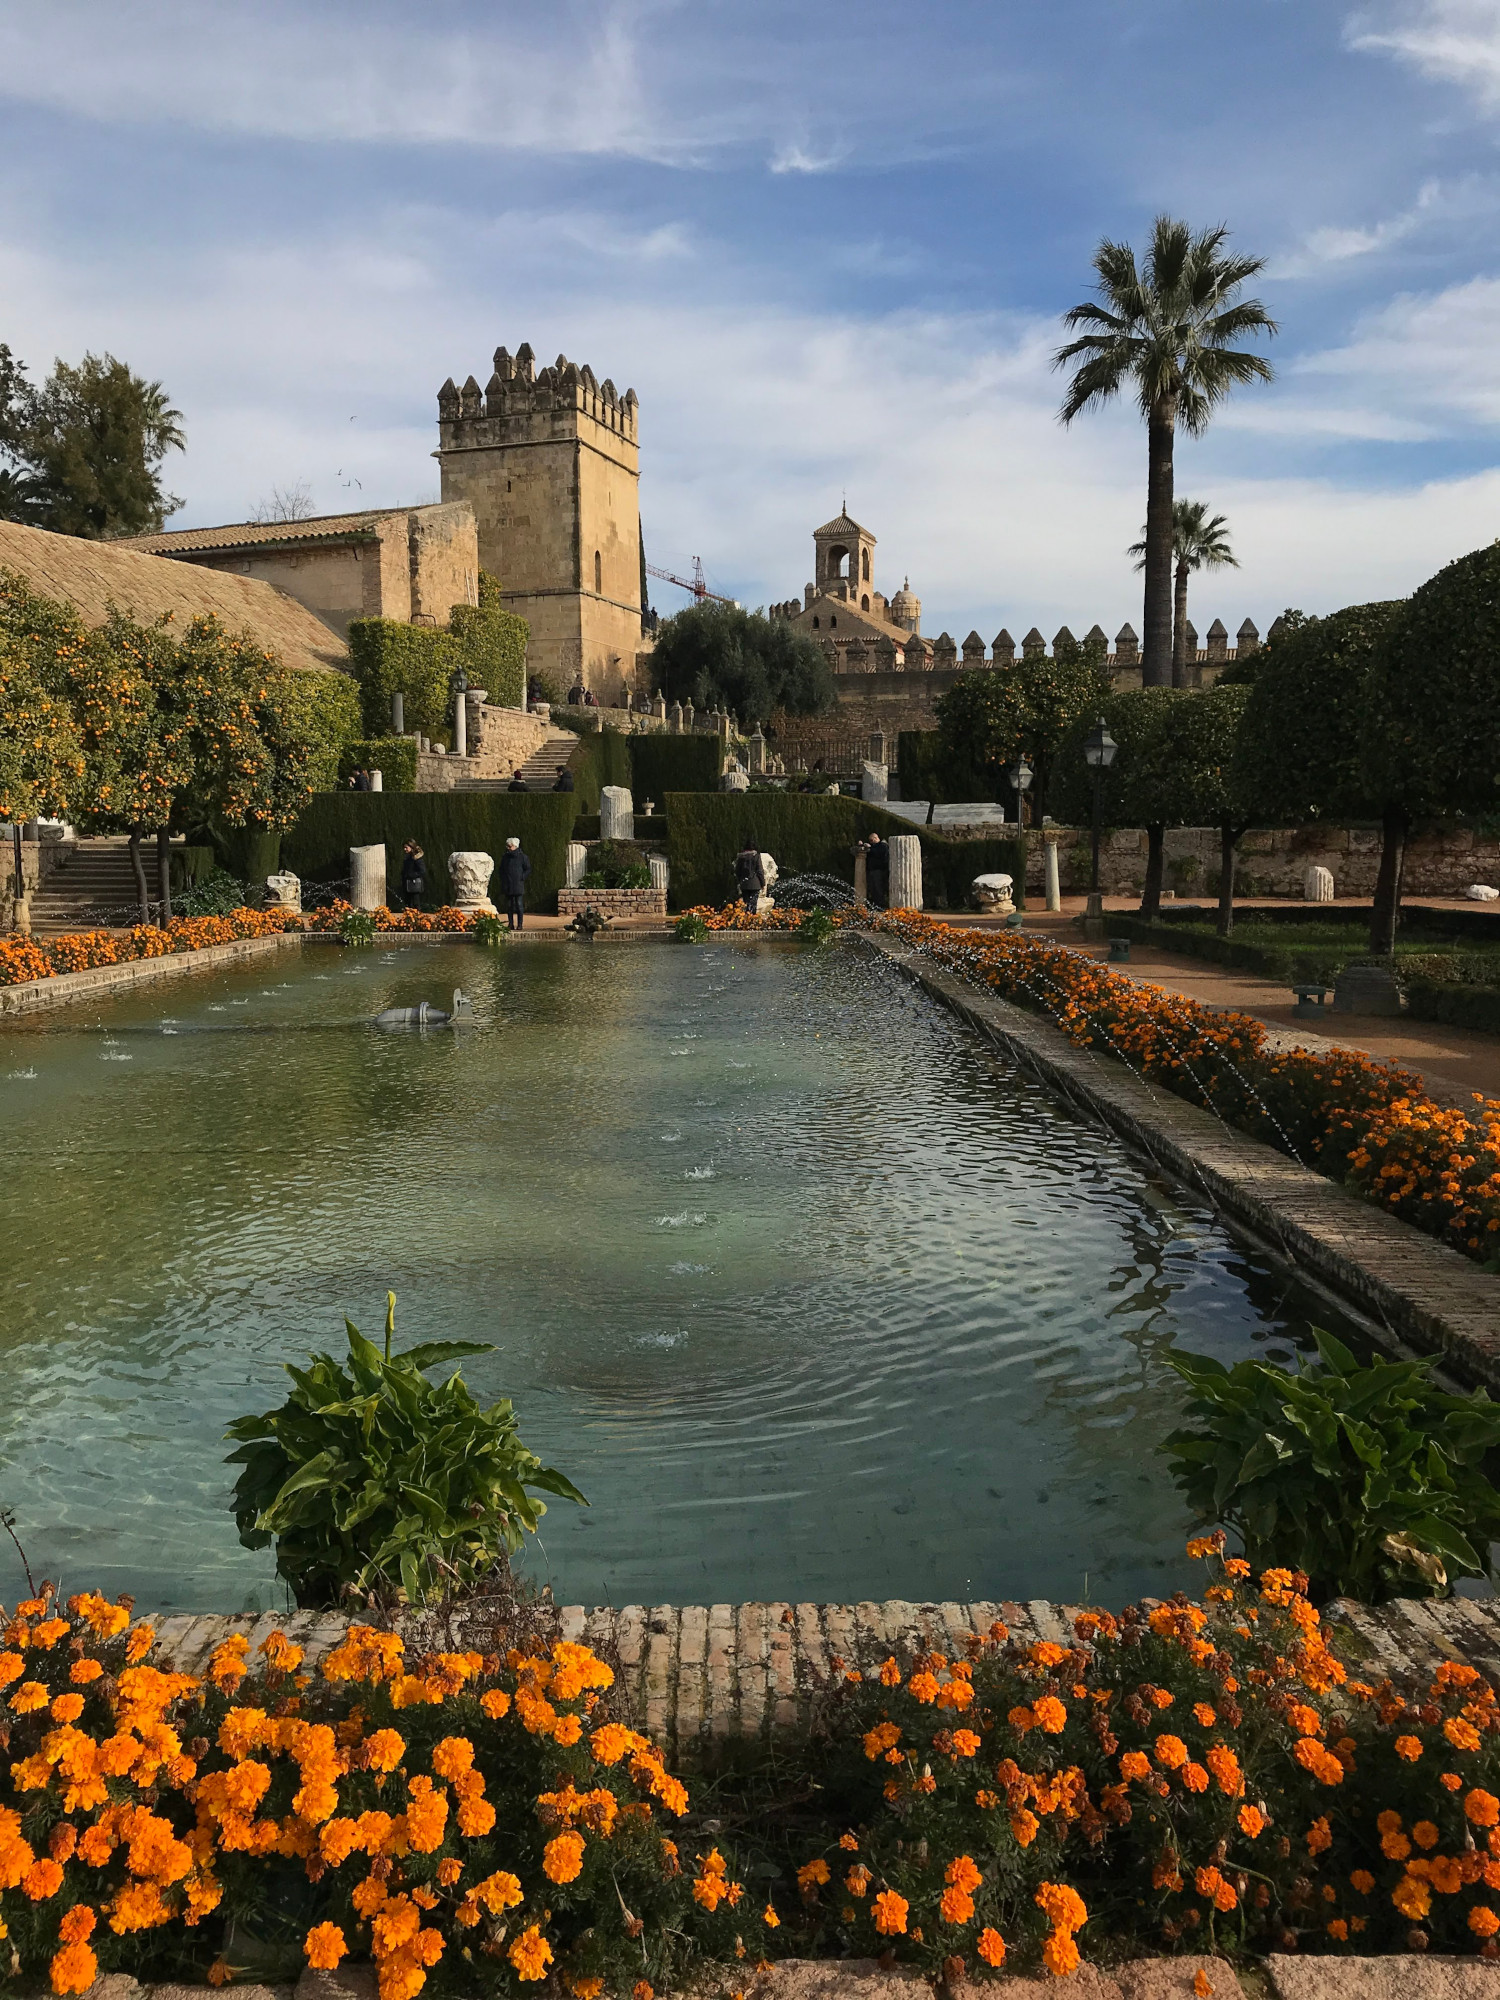
\includegraphics[width=\linewidth]{figures/examples/Alcazar_Cordoba.jpg}
    \caption[Alcázar de los reyes cristianos, Córdoba.]{Alcázar de los reyes cristianos, Córdoba. \href{https://es.wikipedia.org/wiki/Archivo:Alcazar_Cordoba.jpg}{Ahura klik}.}
    \label{fig:apxA:cordoba}
\end{figure}



In vestibulum faucibus ligula eget blandit. Donec eget cursus risus, quis suscipit justo. Curabitur efficitur, dolor nec pulvinar pellentesque, lectus eros hendrerit nisi, in aliquet erat nunc non ipsum. Curabitur felis nunc, viverra nec quam ultrices, suscipit condimentum nibh. Nam faucibus felis hendrerit imperdiet maximus. Curabitur tincidunt porttitor lectus quis feugiat. Sed imperdiet bibendum mi.

\begin{description}
    \item[Nullam quis lacus] vel ante feugiat efficitur id ut quam. Pellentesque commodo elit nec urna gravida maximus. Suspendisse ut risus eu ipsum porta porta ac et orci. Donec dictum ligula sodales, euismod est sed, semper libero \glsname{fiducial}. 
    \item[In blandit], nulla et elementum pharetra, mi nunc sagittis tellus, sit amet scelerisque magna elit ac sapien. Curabitur ipsum dui, pretium a maximus id, varius gravida nisl. Sed vitae mattis elit, vitae hendrerit lorem \cite{IEEE315}.
\end{description}

\subsubsection{Lorem ipsum dolor sit amet, consectetur adipiscing elit}

Integer tempus quis elit id sagittis. Cras tincidunt nisi at tellus luctus, et congue dolor posuere. Aliquam suscipit felis sit amet lacus ultrices aliquet. Sed sagittis ultrices nisi, vel elementum elit dignissim non. 

\subsubsection{Fusce faucibus ex at massa ultrices elementum}

Nullam ullamcorper lorem sit amet facilisis cursus. Suspendisse non erat non justo porta placerat. Morbi porttitor dictum molestie. Sed vitae iaculis libero. Suspendisse in gravida lacus, tempor ultrices nibh. Nam consequat scelerisque porttitor.

\section{Nulla elementum orci in dolor dapibus}

Nulla elementum orci in dolor dapibus, ac facilisis sem ultrices. Nullam eleifend id eros sed luctus. Maecenas arcu ipsum, scelerisque id lorem in, placerat posuere tellus. Etiam gravida velit sed arcu viverra dapibus. Mauris vitae augue dapibus, molestie justo eget, condimentum ipsum. Nulla tristique mi eget semper luctus. Etiam commodo vestibulum vulputate. Etiam quis sapien dolor. Nunc tristique eu lacus quis ullamcorper. Sed volutpat rutrum vehicula. Donec nunc nisl, suscipit in faucibus vitae, tristique eu risus. Nulla facilisis augue eget interdum rutrum. Aliquam sem nunc, fermentum sed urna ac, faucibus interdum nisi.

\subsection{Non luctus mi sollicitudin}

Nam ac tellus ut eros sollicitudin luctus at ac mi. Vestibulum mollis nec nisi a laoreet. Proin neque tortor, placerat nec suscipit sit amet, ullamcorper in sem. Fusce faucibus ultrices cursus. Maecenas scelerisque mauris diam, at volutpat nisi porta vitae. Sed at ipsum et leo cursus varius eu eu lectus. Class aptent taciti sociosqu ad litora torquent per conubia nostra, per inceptos himenaeos. Ut felis ipsum, imperdiet rhoncus orci ac, consectetur luctus nisl. Cras aliquet elementum tellus ullamcorper malesuada. Integer purus est, pharetra eu ullamcorper quis, imperdiet non turpis.

In vestibulum faucibus ligula eget blandit. Donec eget cursus risus, quis suscipit justo. Curabitur efficitur \autoref{code:apx:a:python}, dolor nec pulvinar pellentesque, lectus eros hendrerit nisi, in aliquet erat nunc non ipsum. Curabitur felis nunc, viverra nec quam ultrices, suscipit condimentum nibh. Nam faucibus felis hendrerit imperdiet maximus. Curabitur tincidunt porttitor lectus quis feugiat. Sed imperdiet bibendum mi. Cras aliquet elementum tellus ullamcorper malesuada. Integer purus est, pharetra eu ullamcorper quis, imperdiet non turpis. Sed at ipsum et leo cursus varius eu eu lectus. Class aptent taciti sociosqu ad litora torquent per conubia nostra, per inceptos himenaeos. Curabitur felis nunc, viverra nec quam ultrices, suscipit condimentum nibh. Nam faucibus felis hendrerit imperdiet maximus. Curabitur tincidunt porttitor lectus quis feugiat. 

% [caption={Some Python Code \cite{esp32_devkit_reference_design}}
\begin{code}
\captionof{listing}{Some example large code}
\label{code:apx:a:python}
\begin{minted}{python}
"""
Some interesting python code 
Blah Blah Blah
"""

import numpy as np
from matplotlib import pyplot as plt
from numpy.polynomial import Polynomial as Poly

plt.rcParams["font.family"] = "Libertinus Serif"
plt.rcParams['font.size'] = 14
plt.rcParams['mathtext.fontset'] = 'custom'
plt.rcParams['mathtext.rm'] = 'Libertinus Serif'
plt.rcParams['mathtext.it'] = 'Libertinus Serif:italic'
plt.rcParams['mathtext.bf'] = 'Libertinus Serif:bold'

R510 = 508.3  # Ohms
V5 = 5.018  # Volts

# Open files

nmos_vgs, nmos_vr = np.loadtxt('nmos_ids_vgs.csv', delimiter='\t', unpack=True, skiprows=1)
nmos_sim_vgs, nmos_sim_ids = np.loadtxt('CIC_P0_NMOS_ids_vgs_5.txt', delimiter='\t', unpack=True, skiprows=1)

# Do thingies

nmos_ids = nmos_vr / R510  # Current in resistor
p = Poly.fit(nmos_vgs, nmos_ids, 1)  # Tendency line
print(f"f(x) = {p:unicode}")

# Plot stuff

fig0, ax0 = plt.subplots(figsize=[12, 6])
x = np.linspace(0, 6, 100)

plt.plot(nmos_vgs, nmos_ids, linestyle='none', marker=".", label='Experimental')
plt.plot(nmos_sim_vgs, nmos_sim_ids, linestyle='dashdot', label='Simulation')
plt.plot(x, p(x), linestyle='dashed', label='Tendency')

ax0.grid(True, which='major', color='#DDDDDD', linestyle='-', linewidth=0.6)
ax0.grid(True, which='minor', color='#DDDDDD', linestyle=':', linewidth=0.6)
ax0.minorticks_on()

ax0.legend()

plt.title(r'NMOS, curve $I_{DS}$ / $V_{GS}$')
plt.xlabel(r'$V_{GS}$ (V)')
plt.ylabel(r'$I_{DS}$ (A)')

plt.xlim([0, 6])

# Dont forget to save

plt.savefig("nmos_vgs_ids.pdf")
\end{minted}
\end{code}

